\subsection{Dielectric loss constant}
The dielectric loss constant for a mode ${\rm TE}_{\rm mn}$ is given by equation \ref{eq:dielectric_loss_const}.
\begin{equation}
\alpha _{\rm d}^{\rm (mn)} = \frac{\Delta \bar P _{\rm loss/unit}}{2 \bar P} \approx \frac{\epsilon _{\rm r}''}{\epsilon _{\rm r}'} \frac{\pi}{\lambda} \left(\frac{\Lambda _{\rm mn}}{\lambda}\right)
\label{eq:dielectric_loss_const}
\end{equation}
$\Lambda _{\rm mn}$ and $\lambda$ are given by equations \ref{eq:big-lambda} and \ref{eq:small-lambda}.
\begin{equation}
\Lambda _{\rm mn} = \frac{2 \pi}{k_{\rm z}^{\rm (mn)}} = \frac{\lambda}{\sqrt{1 - \left(\frac{f_{\rm c}^{\rm (mn)}}{f}\right)^2}}
\label{eq:big-lambda}
\end{equation}
\begin{equation}
\lambda = \frac{2 \pi}{k_{\rm 0} \sqrt{\epsilon_{\rm r} \mu_{\rm r}}}.
\label{eq:small-lambda}
\end{equation}
According to \citep{pozar},
\begin{equation}
\epsilon'' = \epsilon' \tan \delta = \epsilon _{\rm r} \epsilon _{\rm 0} \tan \delta.
\end{equation}
Given $\tan \delta = 0.002$, we have
\begin{equation}
\alpha _{\rm d}^{\rm (mn)} \approx \frac{k_{\rm 0} \sqrt{\epsilon_{\rm r} \mu_{\rm r}}}{1000 \sqrt{1 - \left(\frac{f_{\rm c}^{\rm (mn)}}{f}\right)^2}}.
\end{equation}
The dielectric loss constant is plotted for the unimodal frequency band in figure \ref{fig:dielec_loss_const}.
\begin{figure}[h t b p]
\centering
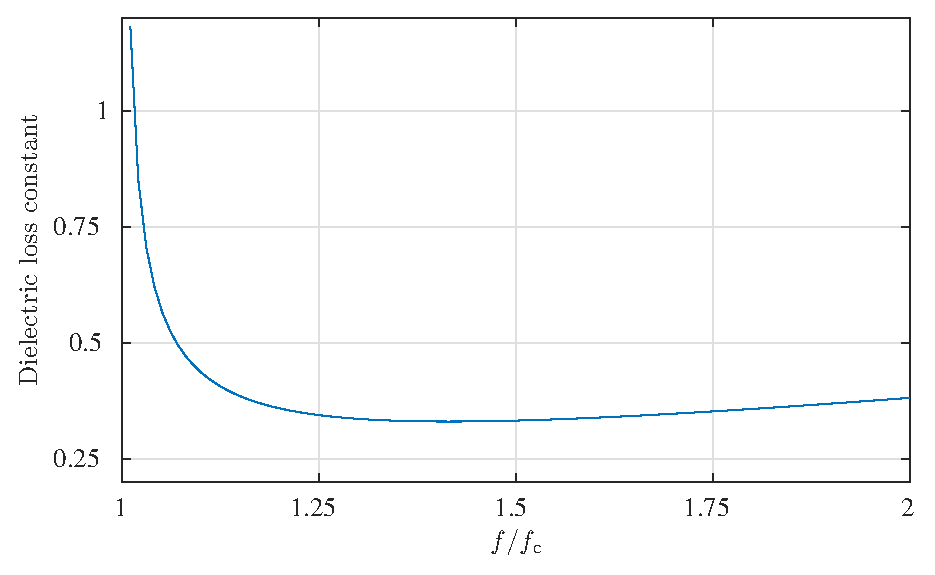
\includegraphics[width=\textwidth,keepaspectratio]{figures/dielec_loss_const.eps}
\caption{Dielectric loss constant, ${\rm TE}_{\rm 10}$ wave.}
\label{fig:dielec_loss_const}
\end{figure}